%\documentclass{article}
%\usepackage{beamerarticle}

\documentclass{beamer}

\usepackage[utf8]{inputenc}
%\usepackage[portuges]{babel}
\usepackage{alltt}
\usepackage{xspace}
\usepackage{longtable}
\usepackage{amsfonts}
\usepackage{latexsym}
\usepackage{amsmath}
\usepackage{amssymb}
%\usepackage{xcolor}
\usepackage{enumerate}
\usepackage{graphicx}
%\usepackage{moreverb}
%\usepackage{ifthen}
\usepackage{url}
\usepackage{tikz} 

%\usetikzlibrary{snakes}
\usetikzlibrary{decorations}
\usetikzlibrary{shapes,shapes.geometric,arrows,fit,calc,positioning,automata,decorations.pathmorphing}
\tikzset{state/.style={draw,ellipse}}

\usepackage{algorithmicx}
\usepackage[noend]{algpseudocode}
\usepackage[Algoritmo]{algorithm}


% \usepackage[utf8]{inputenc}
% %\usepackage[portuges]{babel}
% \usepackage{alltt}
% \usepackage{xspace}
% \usepackage{longtable}
% \usepackage{amsfonts}
% \usepackage{latexsym}
% \usepackage{amsmath}
% \usepackage{amssymb}
% %\usepackage{xcolor}
% \usepackage{enumerate}
% \usepackage{graphicx}
% %\usepackage{moreverb}
% %\usepackage{ifthen}
% \usepackage{url}
% \usepackage{tikz} 

% %\usetikzlibrary{snakes}
% \usetikzlibrary{decorations}
% \usetikzlibrary{shapes,shapes.geometric,arrows,fit,calc,positioning,automata,decorations.pathmorphing}
% \tikzset{state/.style={draw,ellipse}}

% \usepackage{algorithmicx}
% \usepackage[noend]{algpseudocode}
% \usepackage[Algoritmo]{algorithm}

\newcommand{\Versao}{pdf}

\newcommand{\lixo}[1]{}
% VFS6

\newcommand{\REs}{REs\xspace}
\newcommand{\Regfin}{\mathsf{Rfin}\xspace}
\newcommand{\dfa}{DFA\xspace}
\newcommand{\dfas}{DFAs\xspace}
\newcommand{\nfa}{NFA\xspace}
\newcommand{\enfa}{$\varepsilon$-NFA\xspace}
\newcommand{\enfas}{$\varepsilon$-NFAs\xspace}
\newcommand{\nfas}{NFAs\xspace}
\newcommand{\Set}[1]{\{\,#1\,\}}
\newcommand{\fun}{\rightarrow}
 \newcommand{\Implica}{\mbox{$\Rightarrow$}}
 \newcommand{\equival}{\mbox{$\Leftrightarrow$}}
 \newcommand{\halmos}{\mbox{$\Box$} \vspace{0.25in}}
 % \newcommand{\ie}{\mbox{\em i.e.}}
 \newcommand{\prim}{$1^{\mbox{\small \b{a}}}$\ }
 \newcommand{\eira}[1]{$#1^{\mbox{\small \b{a}}}$\ }
 \newcommand{\eiro}[1]{$#1^{\mbox{\small \b{o}}}$\ }
 \newcommand{\num}{$\mbox{n}^{\mbox{\small \b{o}}}$\ }
 % \newcommand{\set}[1]{\{#1\}}
 \newcommand{\Union}{\cup}
 \newcommand{\Inter}{\cap}
 \newcommand{\AND}{\;\land\;}
 \newcommand{\ANDe}{\;\land}
 \newcommand{\Or}{\;\lor\;}
 \newcommand{\Ore}{\;\lor}
 \newcommand{\Imp}{\to}
 \newcommand{\Impv}{\;\to\;}
 \newcommand{\Equiv}{\leftrightarrow}
 \newcommand{\True}{\mathsf{true}}
 \newcommand{\False}{\mathsf{false}}
 \newcommand{\NAND}{\tilde{\AND}}
 \newcommand{\NOR}{\tilde{\Or}}
 \newcommand{\ORE}{\dot{\lor}}
 \newcommand{\bool}{{\cal BOOL}}
 \newcommand{\EEquiv}{\Longleftrightarrow}
 \newcommand{\V}{{\color{red} \textbf{V}}}
 \newcommand{\Fa}{{\color{red} \textbf{F}}}

\newcommand{\Ident}{\equiv}



%MC
\newcommand{\kleene}[1]{\mbox{${#1}^\star$}}
\newcommand{\nter}[1] {\mbox{$\langle #1 \rangle$}}
\newcommand{\deriva}{\Rightarrow}
\newcommand{\produ}{\to}
\newcommand{\blank}{\bullet}
\newcommand{\esqa}{\mbox{$\gets$}}
\newcommand{\dira}{\mbox{$\to$}}

%LC
\newcommand{\Varp}{\mbox{${\cal V}_{Prop}$}}
\newcommand{\suf}{\mbox{$\Rightarrow$}}
\newcommand{\nec}{\mbox{$\Leftarrow$}}
\newcommand{\esimo}[2]{$#1^{\mbox{\small \b{#2}}}$\ }


%SD
\newcommand{\la}{\lambda}
\newcommand{\lc}{$\lambda$-calculus\xspace}
\newcommand{\lt}{$\lambda$-termo\xspace}
\newcommand{\lts}{$\lambda$-termos\xspace}
\newcommand{\LC}{\Lambda(\CC)}
\newcommand{\CLC}{{\cal CL}(\CC)}
\newcommand{\CL}{{\cal CL}}
\newcommand{\lapp}{\backslash}
\newcommand{\Rbu}[2]{ #1\rightarrow_{1\beta} #2 } 
\newcommand{\Rb}[2]{ #1\rightarrow_{\beta} #2 } 
\newcommand{\Ra}[2]{ #1\rightarrow_{\alpha} #2 } 
\newcommand{\Cb}[2]{ #1\equiv_{\beta} #2 } 
\newcommand{\Reu}[2]{ #1\rightarrow_{1\eta} #2 } 
\newcommand{\Ret}[2]{ #1\rightarrow_{\eta} #2 } 
\newcommand{\Ce}[2]{ #1\equiv_{\eta} #2 } 
\newcommand{\Rbeu}[2]{ #1\rightarrow_{1\beta\eta} #2 } 
\newcommand{\Rbet}[2]{ #1\rightarrow_{\beta\eta} #2 } 
\newcommand{\Cbe}[2]{ #1\equiv_{\beta\eta} #2 } 

%FLP

\newcommand{\Rw}{ \mapsto_{w} } 
\newcommand{\Rws}{ \mapsto_{w}^\star } 


\newcommand{\nums}[1]{\lceil\ #1\rceil}
\newcommand{\cpo}{($D$,$\sqsubseteq$)\ }

\newcommand{\cp}[1]{(#1,$\sqsubseteq$)}
\newcommand{\nn}{\mbox{$\mathbb{N}$}}
\newcommand{\nb}{\mbox{$\,\mathbb{N}_\bot\,$}}
\newcommand{\sse}{\Longleftrightarrow}
\newcommand{\ordu}{\sqsubseteq}
\newcommand{\nttr}{\;\nrightarrow\;}
\newcommand{\ttr}{\;\rightsquigarrow\xspace}
\newcommand{\tr}{\longrightarrow\xspace}
\newcommand{\trs}{\;\longrightarrow^\star\xspace}
\newcommand{\trtau}{\;\Rightarrow\;}
\newcommand{\tc}{\;\hookrightarrow\;}
\newcommand{\trd}{\;\rightarrow^d_v\;}
\newcommand{\confd}[2]{\langle #1,#2 \rangle}
\newcommand{\son}[3]{\confd{#1}{#2}\;\tr\;#3}
\newcommand{\sos}[4]{\confd{#1}{#2}\;\tr\;\confd{#3}{#4}}
\newcommand{\transt}[3]{#1\stackrel{#2}{\ttr}#3}
% \newcommand{\trans}[3]{#1\stackrel{#2}{\tr}#3}
\newcommand{\transs}[3]{#1\stackrel{#2}{\trs}#3}
\newcommand{\transc}[3]{#1\stackrel{#2}{\tc}#3}
\newcommand{\transi}[4]{#1\stackrel{#2}{\tr_{#4}}#3}
\newcommand{\transci}[4]{#1\stackrel{#2}{\tc_{#4}}#3}
\newcommand{\transtau}[3]{#1\stackrel{#2}{\trtau}#3}

\newcommand{\sta}[1]{\langle #1 \rangle}
\newcommand{\einf}{\stackrel{\infty}{\exists}}
\newcommand{\ainf}{\stackrel{\infty}{\forall}}
\newcommand{\sap}{(2^{AP})^\omega}
\newcommand{\sas}{(2^{AP})^\star}
\newcommand{\sam}{(2^{AP})^\plus}
\newcommand{\pw}{{\bf P}$\omega$}
\newcommand{\nat} {{\bf N}}
\newcommand{\fnn} {[\nat \longrightarrow \nat]_\bot}
\newcommand{\fff} {\fnn \longrightarrow \fnn}


\newcommand{\Lub}{\bigsqcup}


\newcommand{\rb}{\rightarrow_\beta}
\newcommand{\cb}{=_\beta}
\newcommand{\cbe}{=_{\beta\eta}}
\newcommand{\re}{\rightarrow_\eta}

%\newcommand{\vec}[1]{\overline{#1}}
\newcommand{\lsbra}{[\![}
\newcommand{\rsbra}{]\!]}
\newcommand{\bras}[1]{\lsbra  #1 \rsbra}
\newcommand{\brase}[1]{\lsbra  #1 \rsbra_\Gamma}
%\newcommand{\brass}[1]{Sat(#1)}
\newcommand{\sv}[2]{{\cal #1}\lsbra #2\rsbra}
\newcommand{\svs}[3]{{\cal #1}\lsbra #2\rsbra #3}
\newcommand{\svsc}[3]{{#1}\lsbra #2\rsbra #3}
\newcommand{\svsd}[4]{{#1}\lsbra #2\rsbra #3\, #4}
\newcommand{\svd}[2]{{#1}\lsbra #2\rsbra}
\newcommand{\svr}[3]{#1\lsbra #2\rsbra #3}
\newcommand{\svl}[2]{{\cal #1}\lsbra #2\rsbra\rho}
\newcommand{\svc}[2]{{\cal #1}\lsbra #2\rsbra\varphi\rho}
%\newcommand{\svc}[2]{{\cal #1}\lsbra #2\rsbra\rho\kappa}
%\newcommand{\svt}[2]{{\cal #1}\lsbra #2\rsbra\rho\theta}

\newcommand{\IFF}[3]{#1\,\fun \,#2,#3} 


\newcommand{\namesn}[1]{{#1}_{sn}}
\newcommand{\namess}[1]{{#1}_{ss}}
\newcommand{\namesd}[1]{{#1}_{sd}}

\newcommand{\fixp}[1] {\textsf{FIX}\; #1}

%VFS


\newenvironment{inducao}[2]{
  \begin{description}
      \setlength{\itemsep}{0cm}\setlength{\parsep}{0cm}
    \item[{\em Base.}] #1
    \item[{\em Indução.}] #2}
    {\end{description}}

\newenvironment{inducaoi}[1]{
    \begin{description}
      \setlength{\itemsep}{0cm}\setlength{\parsep}{0cm}
    \item[{\em Indução.}] #1}
    {\end{description}}

\newenvironment{inducaob}[1]{
    \begin{description}
      \setlength{\itemsep}{0cm}\setlength{\parsep}{0cm}
    \item[{\em Base.}] #1}
    {\end{description}}


\newenvironment{pequeno}{

\small

}{}

\newenvironment{mini}{

\tiny

}{}


 \newenvironment{twocol}[4]{

  \begin{tabular}{l|l}
    \begin{minipage}[t]{#1cm}
#2
    \end{minipage}
&
    \begin{minipage}[t]{#3cm}
#4
\end{minipage}
\end{tabular}
}{}






\newcounter{cont}
\newcounter{conti}

\newenvironment{dem}{{\bf Dem:} }

\newenvironment{proofu}{\setlength{\topsep}{-0.3cm}\setlength{\partopsep}{-0.3cm}\begin{description}\item[Dem.] }{\hfill $\Box$ \bigskip
\end{description}}

 \newenvironment{resolv}[1]{
 {\bf Resolução #1}

 }{}

 \newenvironment{coment}[1]{
 {\bf Comentário #1}

 }{}


\newenvironment{exerc}{\begin{exe} \it }{ 
$\diamond$ \end{exe}}

\newenvironment{exercicio}{\begin{Ex} \em }{ 
 \end{Ex}}

\newenvironment{resposta}[1]{{\parbox[t]{14cm}{{\bf R:}
  \vspace*{#1}}}}

\newenvironment{resposta1}[1]{{\parbox[t]{8cm}{{\bf R:} \vspace*{#1}}}}

\newcounter{taben}

\newenvironment{tabenum}{
\begin{enumerate}
  \setcounter{enumi}{\value{taben}}
  \renewcommand{\labelenumi}{\arabic{enumi}.}
  \renewcommand{\theenumi}{\arabic{enumi}.} }{\setcounter{taben}{\value{enumi}}\end{enumerate}}

%\usepackage{aula}

\newcounter{aula}

\newtheorem{exe}{Exercício}[aula]
\newtheorem{exem}{Exemplo}[aula]
\newtheorem{Ex}{Ex}[aula]
 \newtheorem{prob}{Problema}[aula]
 \newtheorem{lema}{Lema}[aula]
 \newtheorem{resol}{Resolução}[aula]
\newtheorem{teor}{Teorema}[aula]
\newtheorem{Def}{Definição}[aula]

\newtheorem{propos}{Proposição}[aula]
\newtheorem{cor}{Corolário}[aula]

%\newenvironment{saida}[1]{\fbox{\begin{verbatim} #1}{\end{verbatim}}}


\newcommand{\apply}{\textsc{apply}}
\newcommand{\restrict}{\textsc{restrict}}
\newcommand{\reduce}{\textsc{reduce}}
\newcommand{\foral}{\textsc{forall}}
\newcommand{\exist}{\textsc{exists}}


%\setlength{\itemsep}{0cm}

\tikzstyle{st}=[state, rectangle, rounded corners=7pt,  inner sep=4pt, minimum size=14pt]










\usepackage{hyperref}

\mode<presentation>
{
   \usetheme{Pittsburgh}
 %\usetheme{Montpellier}
  % or ...
 \usecolortheme{beaver}
  \setbeamertemplate{navigation sysmbols}{}


  \setbeamercovered{transparent}
  % or whatever (possibly just delete it)
}

\mode<handout>{
\usepackage{pgfpages}
\pgfpagesuselayout{2 on 1}[a4paper,border,shrink=5mm] 

}
\setlength{\parindent}{0.0in} 
\setlength{\parskip}{0.05in}
%\MyLogo{Departamento de Ciência de Computadores da FCUP --- LC --- Aula \theaula}

%\rightfooter{\thepage}

\title{Programação Concorrente}
\author[N.~Moreira/ J.~Proença]{Nelma Moreira e José Proença}

\institute[DCC-FC]{Departamento de Ciência de Computadores da FCUP}

\date[Aula \theaula]{Programação Concorrente \\ Aula \theaula}


 \begin{document}

\setcounter{aula}{1}
%\tableofcontents
\section*{Aula \theaula}

\begin{frame}
  \titlepage
\end{frame}

\section{Programação Concorrente CC3037}

\begin{frame}
\frametitle{Objectivos}
\begin{itemize}
	\item descrição formal dos conceitos básicos de concorrência e sua aplicação
\item raciocinar sobre a  correção de programas concorrentes  em relação a especificações
\item desenho e análise de programas concorrentes
\end{itemize}	
\end{frame}

\begin{frame}
\frametitle{Parte 1}
\begin{itemize}
\item	Conceitos básicos de programação concorrente
\item Noções básicas de concorrência
\item Sistemas de transições
\item CCS: \emph{Calculus of Communicating Systems}:
sequência, composição, sincronização;
restrição e reetiquetagem;
parâmetros e dados
\item Comportamento observável
\begin{itemize}
\item relações de equivalência, congruência, bisimulações; 
\item congruência observável
\item propriedades algébricas
\end{itemize}
\item Problemas de sincronização: exclusão mútua, deadlock, locks, etc.
%\item pseuCo: linguagem de programação para agentes concorrentes
%\begin{itemize}
%\item pseuCo e CCS
%\item cooperação por passagem de mensagens (canais síncronos e assíncronos)
%\item cooperação por partilha de memória
%\item primitivas de sincronização (exclusão mútua, semáforos, locks, barreiras e monitors)
%\end{itemize}
\end{itemize}
\end{frame}

\begin{frame}{Bibliografia e Software}
	\begin{itemize}
		\item Reactive systems modelling, specification and verification. Luca Aceto, Anna Ingólfsdóttir, Kim Guldstrand Larsen, Jiri Srba
2007 (Cap. 1-4 e 7)
\item Introduction to Concurrency Theory.
Roberto Gorrieri and Cristian Versari
2015
\item Communication and Concurrency, Robin Milner.
 Prentice Hall International Series in Computer Science, 1989.
\item Modelação usando simuladores de CCS, p.e.: 
  \begin{itemize}
  \item \href{https://pseuco.com}{pseuco.Com}
    \item \href{http://caal.cs.aau.dk}{CAAL}
\end{itemize}
\end{itemize}
\end{frame}


\begin{frame}{Concurrent Programming - Part II}

\includegraphics[width=350pt]{1-intro-slide2.pdf}
%Topics:
%\begin{itemize}
%\item {\bf Classical concurrency problems.} 
%Mutual exclusion, deadlock, starvation, race conditions, atomicity. 
%\item {\bf The thread model}. 
%Shared memory and thread-based concurrency primitives in Java.
%Heisenbugs, validation through (special forms of) testing.
%\item {\bf Concurrent objects / data structures.}
%Linearizability of concurrent objects.
%Lock-based vs. lock-free implementations.
%\item {\bf Other concurrency models.}
%Message-passing concurrency using the actor model.
%Software Transactional Memory (STM).
%Brief overview of actor and STM programming in Scala.
%\end{itemize}
\end{frame}



\begin{frame}

\frametitle{Programação Concorrente- CC3040}

 \textbf{Páginas Web} 

\textbf{Sigarra: \url{}}

\textbf{URL Geral:} \url{https://moodle2425.up.pt/}\\

\textbf{Específicas}:
\begin{description}
	\item 

\textbf{Parte 1:}

\url{https://www.dcc.fc.up.pt/~nam/Teaching/progcon2425/}

Pass: \alert{RobinMilner}

\item \textbf{Part II:}

\url{https://fm-dcc.github.io/pc2425/}
\end{description}

\textbf{Email}: institucional

\textbf{Escolaridade:} $2$T e $2$PL

\textbf{Frequência:} $3/4$ de presenças nas aulas PL e $>6$ em $20$ no trabalho prático.
\end{frame}
\begin{frame}
    \begin{block}{Método de avaliação}

 \begin{enumerate}
\item Avaliação distribuída sem exame final
\item  2 Testes (70\%)  e trabalho (30\%)
\item  Cada Teste: (35\%) e (nota mínima: 6 valores em 20)
\item Exame de recurso: 70\% + Trab (30\%)
\item Exame de melhoria: 100\% 
\end{enumerate}
\end{block}
{\Large \alert{Teste 1}: 12/04/2025 9h}
\end{frame}


\begin{frame}
\frametitle{Programas Sequenciais}
\begin{itemize}
	\item realizam uma função dos dados nos resultados (tese de Church/Turing)

\item A sua semântica pode ser analisada considerando o estado (memória) em cada instante:
$$\sv{S}{P}: State \fun State$$
onde p.e. $State=[Var \fun \mathbb{Z}]$.

$P:$
\begin{algorithmic}
\State $x\gets 1$
\State $y\gets 0$
\While{$x<10$}
\State $y \gets y+x$
\State $x \gets x+1$
\EndWhile
\State \textbf{print} $y$
\end{algorithmic} 
\item Terminam (se não terminarem a sua semântica é indefinida)
\end{itemize}	
\end{frame}

\begin{frame}[fragile]
\frametitle{Equivalência de programas sequenciais}

\only<1->{\emph{Dois programas são equivalentes se realizam a mesma função.}
}
\only<2->{	
\begin{columns}
	\begin{column}[t]{0.3\textwidth}
$P:$
\begin{algorithmic}
\State $x\gets 1$
\end{algorithmic}
\end{column} 
\begin{column}[t]{0.5\textwidth}
$Q:$
\begin{algorithmic}
\State $x\gets 0$
\State $x\gets x+1$
\end{algorithmic} 
\end{column}
\end{columns}}

\only<3->{
$P$ e $Q$ são equivalentes assim como  são equivalentes a 
\begin{itemize}
	\item $P;Q$
\item  $Q;P$ 
\item $R;P$ e $R;Q$ (para qualquer programa $R$)
\item $\ldots$
\end{itemize}}
\only<4->{
A semântica de programas sequênciais é composicional. Por examplo a semântica de $P;Q$ é obtida da semântica de $P$ e de $Q$.}
\end{frame}

\begin{frame}
	\frametitle{Programas Sequênciais vs Concorrentes}
\begin{columns}
	\begin{column}[t]{0.3\textwidth}
$P:$
\begin{algorithmic}
\State $x\gets 1$
\end{algorithmic}
\end{column} 
\begin{column}[t]{0.5\textwidth}
$Q:$
\begin{algorithmic}
\State $x\gets 0$
\State $x\gets x+1$
\end{algorithmic} 
\end{column}
\end{columns}

\begin{itemize}[<+->]
	\item Mas se os executarmos em paralelo, $P || Q$?
\item Qual o significado? $P$ e $Q$ podem intercalar
\begin{enumerate}
	\item não é único: 
\begin{itemize}
\item pode ser  $1$: se for $P$ e depois $Q$
\item  ou $2$: se for $Q$ (primeira instrução) , depois $P$ e depois $Q$ (segunda instrução)
\end{itemize}
\item a semântica não é determinística
\item a equivalência não é preservada por $||$.
\item não é composicional (a semântica de um composta com a semântica do outro)
\end{enumerate}
\end{itemize}
\end{frame}

\begin{frame}
	

\frametitle{Programas Concorrentes/Sistemas Reactivos}
\begin{itemize}%[<+->]
	\item Normalmente não calculam uma função
 \begin{itemize}
\item  Sistemas de operação 
\item Protocolos de comunicação
\item Sistemas Web
\item Sistemas embebidos
\item Processadores multicore
\item Sistemas de controlo de tráfego
\item Portagens
\item $\cdots$
\end{itemize}
\item Então o que fazem?
\item Interagem com o ambiente e entre eles, trocando informação.
\item Normalmente não terminam.
\item Componentes básicas: Processos ou Agentes
\end{itemize}
\end{frame}

\begin{frame}
	

\frametitle{Concorrência vs Paralelismo}
\alert{Concorrência}
\begin{columns}
\begin{column}{0.5\textwidth}
	\begin{itemize}
\item Trabalho lógico simultaneo 
\item Não obriga a multiprocessador
\end{itemize}
\end{column}
	\begin{column}{0.5\textwidth}
	 \includegraphics[width=6cm]{IMG/concurnotpar}
\end{column}
\end{columns}
\pause
\alert{Paralelismo}
	\begin{columns}
\begin{column}{0.5\textwidth}
	\begin{itemize}
\item Trabalho físico simultaneo 
\item Obriga a multiprocessador ou várias unidades de processamento.
\end{itemize}
\end{column}
	\begin{column}{0.5\textwidth}
	 \includegraphics[width=6cm]{IMG/concurpar}
\end{column}

\end{columns}

\end{frame}

\begin{frame}
	

\frametitle{Processos}

\begin{itemize}[<+->]
	\item Um \alert{processo} é  um programa (sequencial) em execução
\item É descrito por uma máquina de estados (estado= memória, contador de programa, etc)
\item Um \alert{programa multiprocesso} comporta-se como um conjunto de máquinas de estados que cooperam através  da comunicação com o meio.
\item se cada processo tiver um processador, os processos podem executar em paralelo
\item Senão, tem de haver um \alert{escalonador}  para atribuir processos a processadores
 \item Supomos sistemas asíncronos onde \alert{o tempo de execução não interessa}

\end{itemize}
\end{frame}

\begin{frame}
\frametitle{Sincronização de Processos}	
\begin{itemize}[<+->]
	\item Quando o progresso de um ou mais  processos depende do comportamento de outros processos
\item As interações podem ser de dois tipos:
\begin{enumerate}
\item competição 
\begin{itemize}
\item Ex: competição por um recurso partilhado
\end{itemize}
 \item cooperação

\begin{itemize}
\item O progresso de um processo depende do progresso de outros
\item Ex: \emph{rendezvous}: conjunto de pontos de controlo em que cada processo só pode avançar quando todos os processos estiverem no ponto de controlo respectivo.
\item Ex: \emph{produtor/consumidor}
\end{itemize}
 
\end{enumerate}
\end{itemize}

\end{frame}



\begin{frame}
\frametitle{Competição: Ler e escrever num disco $D$}	
%
\begin{columns}
\begin{column}{0.5\textwidth}
\begin{algorithmic}
\Procedure{disk-read}{$x$}
\State{$D.seek(x);$}
\State{$r\gets D.read();$}
\State{\textbf{return} $r$;}
\EndProcedure
\end{algorithmic}
\end{column}
\begin{column}{0.5\textwidth}
\begin{algorithmic}
\Procedure{disk-write}{$x$,$v$}
\State{$D.seek(x);$}
\State{$D.write(v);$}
\State{\textbf{return};}
\EndProcedure
\end{algorithmic}
\end{column}
\end{columns}
\bigskip
\pause

\begin{center}
\begin{algorithmic}
\Call{disk-read}{$x$} $||\;$ \Call{disk-write}{$y$,$v$} 
\end{algorithmic}
\only<2->{
\includegraphics[width=7cm]{IMG/readwrite}}

\pause Pode acontecer que se leia em $x$ o valor de $y$.

\pause \alert{Solução}: Não permitir que estas operações executem em simultaneo $\Imp$ \alert{Exclusão Mútua}  
\end{center}
\end{frame}


\begin{frame}
\frametitle{Cooperação:produtor/consumidor}	

\begin{itemize}[<+->]
	\item O produtor \alert{produz} produtos
\item O consumidor \alert{consume} os produtos, e
\item Um produto não pode ser consumido \alert{antes} de ser produzido
\item Todos os produtos que são produzidos são consumidos  \alert{exactamente} uma  vez
\item Implementação: um \emph{buffer} partilhado de tamanho $k\geq 1$
\item Pode ser uma fila: o produtor acrescenta um novo produto no \alert{fim} da fila e o consumidor consome o produto do \alert{início} da fila
\item O produtor tem de esperar quando o buffer \alert{está cheio}
\item O consumidor só tem de esperar quando o buffer \alert{está vazio}
\item \alert{Invariante de sincronização}: se $\#p$ número de produtos produzidos e $\#c$ número de produtos consumidos:
$$ (\#c\geq 0)\land    (\#p\geq \#c)\land  (\#p\leq \#c+k)$$
\end{itemize}
	
\end{frame}


\begin{frame}
\frametitle{Exclusão Mútua}	
\begin{itemize}[<+->]
	\item \alert{Secção Crítica}: porção de código que só pode ser executado por um processo num dado instante
\item Supõe-se que a execução da secção crítica por um só processo termina.
\item \alert{MUTEX}  o problema consiste em ter
\begin{enumerate}
	\item  um algoritmo de entrada $acquire\_mutex()$
\item um algoritmo de saída $release\_mutex()$
\end{enumerate}
\item Enquadrando a seção crítica garantem
\begin{description}
	\item[Exclusão mútua]: que o código da zona crítica é executado no máximo por um processo em cada instante.
\item[\emph{Starvation-freedom}]: cada processo que invoca $acquire\_mutex()$ termina, permitindo assim que os processos que querem entrar na zona crítica o possam fazer.
\end{description}
\end{itemize}
\end{frame}

\begin{frame}
\frametitle{Exclusão Mútua}	
 \begin{algorithmic}
 \Procedure{$protected\_code$}{$in$}
\State \Call{$acquire\_mutex$}{\ };
\State $r\gets cs\_code(in)$;
\State \Call{$release\_mutex$}{\ };
\State{\textbf{return} $r$;}
\EndProcedure
 \end{algorithmic}
\end{frame}


\begin{frame}
\frametitle{Propriedades de \emph{Safety} e \emph{Liveness}}	
\begin{description}[<+->]

	\item[\emph{Safety} (segurança)] Nada de mal acontece. Podem ser invariantes. Têm de ser sempre verdade. Ex: Exclusão mútua
	\item[\emph{Liveness} (vivacidade)] Algo de bom irá acontecer. Terão de acontecer ao longo da execução do sistema. 
\begin{itemize}
	\item \alert{Starvation-freedom} 
\item \alert{Deadlock-freedom}: em cada instante $\tau$ se vários processos invocaram $acquire\_mutex$ e essa invocação não terminou, então para $\tau'>\tau$ algum terá que terminar essa invocação.

\item \alert{Bypass limitado}: Suponhamos $n$ processos em competição e suponhamos que um  ganha. Existe $f(n)$ tal que cada processo que invoca $acquire\_mutex$ perde no máximo $f(n)$ vezes para os outros.
\end{itemize}
\centerline  \emph{Bypass} limitado $\Imp$ \emph{Starvation-freedom}(=\emph{Bypass} finito) $\Imp$ \emph{Deadlock-freedom}
\end{description}
\end{frame}

\section{Modelação de Sistemas Concorrentes}
\only<presentation>{\begin{frame}
	\frametitle{Modelação de Sistemas Concorrentes}
	Pretendemos modelar os sistemas concorrentes/reactivos de modo a
	\begin{itemize}
		\item  poder assegurar as propriedades indicadas
		\item garantir a sua correção
		\item determinar se uma implementação está de acordo com a especificação
		\item em geral é díficil compreender o comportamento de um sistemas concorrentes
	\end{itemize}
\end{frame}}
\begin{frame}{Máquina de Vendas}
\begin{columns}\begin{column}{0.5\textwidth}
	\includegraphics[width=5cm]{IMG/vendingmachine}	
\end{column}

\begin{column}{0.5\textwidth}
\textbf{Acções de comunicação} (\alert{observáveis})
	\begin{itemize}
		\item Pressionar um botão
\item Inserir moedas
\item Injectar uma bebida/comida
	\end{itemize}
\pause \textbf{Acções internas}

(\alert{ não observáveis})
\begin{itemize}
		\item Escolher a bebida
\item Mecanismo para injectar o produto certo
\item Tirar o dinheiro do bolso
\item Verificar as moedas inseridas
\item Pegar na bebida
	\end{itemize}

\end{column}
	\end{columns}

\end{frame}

\begin{frame}{Modelo abstracto de um processo}

\begin{itemize}[<+->]
	\item Um processo é descrito usando um conjunto de ações, \alert{alfabeto do processo}
\item $Com$: conjunto de ações de comunicação (actividades observáveis) $a,b,c,\ldots$
\item $Int$: conjunto de acções internas (computações locais)   $[a],[b],[c],\ldots$
\item  $Act=Com\cup Int$ conjunto de todas as ações
\item A execução de uma \alert{ação} muda o estado do processo:
 \only<6>{
\begin{center}
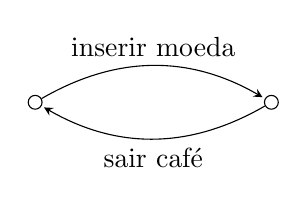
\begin{tikzpicture}[>=stealth, shorten >=1pt, auto, node distance=3cm,initial text={}]
\node[state,  inner sep=1pt, minimum size=5pt] (S0){};
\node[state,  inner sep=1pt, minimum size=5pt][right of =S0] (S1){};
\path[->](S0) edge [bend left] node {inserir moeda}(S1)
         (S1) edge  [bend left] node { sair café}(S0);
\end{tikzpicture}
\end{center}
}

\only<7>{
\begin{center}
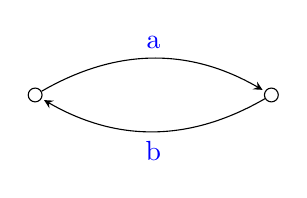
\begin{tikzpicture}[>=stealth, shorten >=1pt, auto, node distance=3cm,initial text={}]
\node[state,  inner sep=1pt, minimum size=5pt] (S0){};
\node[state,  inner sep=1pt, minimum size=5pt][right of =S0] (S1){};
\path[->](S0) edge [bend left] node {\color{blue} a}(S1)
         (S1) edge  [bend left] node { \color{blue}b}(S0);
\end{tikzpicture}

Usar só letras para simplificar
\end{center}
}
\end{itemize}
	
\end{frame}

\section{Sistemas de Transição}

\begin{frame}{Constituintes de um processo}
\begin{itemize}
	\item Um conjunto de estados
\item Um conjunto de transições entre estados
\item Um estado inicial
\item Cada transição é etiquetada por uma ação que  acciona a mudança de estado.
\end{itemize}
	
\end{frame}

\begin{frame}{}
\begin{block}{Estados}
	\begin{itemize}[<+->]
		\item Cor actual de um semáforo de trânsito
\only<1>{\includegraphics[width=3cm]{IMG/traffic-light-red}}
\item Valor corrente das variáveis de um programa e do contador de programa
\item A avião a voar
\item Valor da conta bancária
	\end{itemize}
\end{block}
\pause
	\begin{block}{Transições}
	\begin{itemize}[<+->]
		\item Passagem de  um semáforo de trânsito de vermelho para verde
\item Execução de um comando num programa
\item Aterragem de um avião
\item Depositar dinheiro numa conta bancária
	\end{itemize}
\end{block}
\end{frame}
\begin{frame}{Sistemas de transição}
\begin{Def}
	Um sistema etiquetado de transições (LTS) sobre $Act$ é um triplo $(S,\tr,s_0)$ 
\begin{itemize}
	\item $S$ conjunto de estados
\item $\tr\subseteq S\times Act \times S$ a relação de transição
\item $s_0\in S$ estado inicial
\end{itemize}
\end{Def}
	\only<2->{ Um Fósforo...
\begin{center}
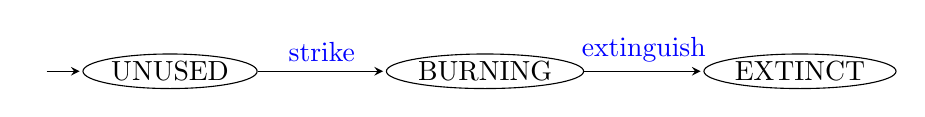
\begin{tikzpicture}[>=stealth, shorten >=1pt, auto, node distance=4cm,initial text={}]
\node[state,  initial,inner sep=1pt, minimum size=5pt] (S0){UNUSED};
\node[state,  inner sep=1pt, minimum size=5pt][right of =S0] (S1){BURNING};
\node[state,  inner sep=1pt, minimum size=5pt][right of =S1] (S2){EXTINCT};

\path[->](S0) edge  node {\color{blue} strike}(S1)
         (S1) edge   node { \color{blue} extinguish }(S2);
\end{tikzpicture}
\end{center}
}
\only<3->{
\begin{itemize}
	\item $S=\{UNUSED,BURNING, EXTINCT\}$
	\item $act=\{strike, extinguish\}$
\item $\tr=\{(UNUSED,strike, BURNING), (BURNING, extinguish, EXTINCT)\}$
\item $s_0=UNUSED$ 
\end{itemize}
}
\end{frame}
\begin{frame}{Sucessores}

Em vez de $(s,\alpha,s')\in \tr$ escrevemos $\trans{s}{\alpha}{s'}$ e dizemos que $s'$ é um   \alert{sucessor} de $s$, sendo $\alpha\in Act$ uma ação.
\begin{itemize}[<+->]
	\item $Post(s,\alpha)=\{\;s'\in S\mid \trans{s}{\alpha}{s'}\;\}$
\item $Post(s,A)=\bigcup_{\alpha\in A} Post(s,\alpha)$, $A\subseteq Act$
\item $Post(s)= Post(s,Act)$
\item$Post(C,\alpha)=\bigcup_{s\in C} Post(s,\alpha)$, $C\subseteq S$
\item $Post(C,A)=\bigcup_{\alpha\in A} Post(s,\alpha)$
\item Ações que ocorrem no estado $s$
$$Act(s)=\{\alpha\in Act\mid \exists s': \trans{s}{\alpha}{s'}\}$$
\item Ações que podem ser observadas no estado $s$
$$Com(s)=\{\alpha\in Com \mid \exists s': \trans{s}{\alpha}{s'}\}$$
\item Análogo para $Int(s)$
\end{itemize}
	\end{frame}
\only<presentation>{\begin{frame}{Um Telefone}}
\only<article>{\begin{frame}{}
\begin{example}\ Considera a seguinte simulação de um Telefone}
\begin{center}
\includegraphics[width=7cm]{IMG/telefone}
\end{center}
\begin{itemize}[<+->]
\item Descreve o sistema de transições $(S,\tr,s_0)$ e $Act=Com\cup Int$.
\item  Alguns exemplos: $Post(RINGING,Act)=\pause\{TALKING, IDLE,OFF\} $
\item 	$Post(Post(RINGING,Act),Int)=\pause\{OFF\} $
\item $Com(RINGING)=\pause\{accept,reject\_call\}$
\end{itemize}
	\only<article>{
	Temos que 
	\begin{align*}S&=\{RINGING, TALKING,IDLE,OFF,PLAYING\}\\
	s_0&=OFF\\
	Com&=\{accept,reject_call,incoming\_call,switch\_on,switch\_off,dial,\\& end\_call, load\_game, game\_over\}\\
	Int&=\{[battery\_low]\}\\
	Act&=Com \cup Int\\
	\tr&=\{ (OFF,switch\_on,IDLE), (IDLE, incoming\_call, RINGING),\\& (IDLE, [battery\_low], OFF),  (IDLE, dial, TALKING), \ldots\} 
	\end{align*}
	Podes completar indicando $Act(IDLE)$.
\end{example}}
\end{frame}

\begin{frame}{Estados atingíveis}
	\begin{itemize}
		\item Seja $TS=(S,\tr,s_0)$ um LTS. 
		\item Um estado $s'\in S$ é \alert{atingível} de $s$ se $s'=s$  ou
\item 
$\exists n\geq 0$ e estados $s_1,s_2,\ldots , s_n$ tal que
$\trans{s}{\alpha_1}{s_1}\trans{}{\alpha_2} {s_2}\;\cdots\trans{}{\alpha_n}{s_n}$ e $s_n=s'$.
\item neste caso diz-se que existe um caminho de tamanho $n$ entre $s$ e $s'$ 
\item um caminho  é \emph{acíclico} se $s_i\not=s_j$ para todo $i\not=j$; caso contrário diz-se cíclico.

\item $Reach(s)$ conjunto de estados atingíveis de $s$
\item $Reach(TS)=Reach(s_0)$

\end{itemize}
Sendo $\trs\subseteq S\times Act^\star \times S$ o fecho reflexivo e transitivo de $\tr$,  então  $
\transs{s}{\omega}{s'}$ se e só se $s'\in Reach(s)$, onde $\omega=\alpha_1\cdots \alpha_n$ para alguns $\alpha_i\in Act$.
\only<article>{
\begin{exerc}
	Mostra a afirmação anterior.
\end{exerc}}
\end{frame}
\section{Não-determinismo}
\begin{frame}{Não-determinismo}
	\begin{columns}
\begin{column}{0.6\textwidth}
	\begin{itemize}[<+->]
		\item Permite descrever o comportamento de sistemas reais
\item Abstração de detalhes dos sistemas
\begin{itemize}
\item não é necessária uma descrição completa
\item os sistemas podem ser muito complexos
\item alguns parâmetros são desconhecidos
	\end{itemize}
\item existem várias maneiras de interagir
\item a noção é mais geral que em Linguagens Formais
\end{itemize}
\end{column}
	\begin{column}{0.4\textwidth}
	\includegraphics[width=5cm]{IMG/telefone}
\end{column}
\end{columns}

\end{frame}
\begin{frame}{} %{Não-determinismo}
\begin{itemize}[<+->]
	\item Seja $TS=(S,\tr,s_0)$ um LTS. 
\item $TS$ é \alert{determinístico} se e só se para todo $s\in S$
\item $|Post(s)|\leq 1$ e $|Act(s)|\leq 1$
\item senão é \alert{não-determinístico}
\end{itemize}
\only<4>{
\begin{columns}
\begin{column}{0.5\textwidth}
	Um sistema é não determinístico se tem um estado com duas ou mais transições mas não sabemos qual irá acontecer.

\end{column}
	\begin{column}{0.5\textwidth}
	\includegraphics[width=6cm]{IMG/telefone}
\end{column}
\end{columns}}


\end{frame}

\begin{frame}{Não-determinismo interno e externo}
Um  estado $s$  é
\begin{itemize}[<+->]
	\item não-determinístico \alert{externo} sse $|Com(s)|> 1$
\item não-determinístico \alert{interno} sse $|Post(s,Int)|> 1$ ou  $|Post(s,a)|> 1$ para algum $a\in Com(s)$ 
\end{itemize}
\end{frame}
\begin{frame}[fragile]{Não-determinismo interno e externo}\begin{center}
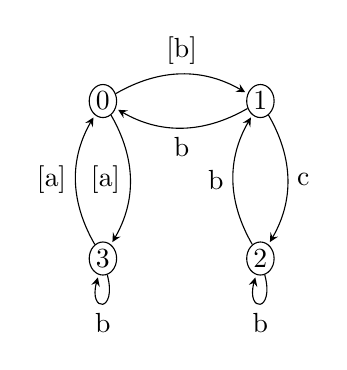
\begin{tikzpicture}[>=stealth, shorten >=1pt, auto, node distance=2cm,initial text={}]
\node[state,  inner sep=1pt, minimum size=5pt] (S0){0};
\node[state,  inner sep=1pt, minimum size=5pt][right of =S0] (S1){1};
\node[state,  inner sep=1pt, minimum size=5pt][below of =S0] (S3){3};
\node[state,  inner sep=1pt, minimum size=5pt][below of =S1] (S2){2};
\path[->](S0) edge [bend left, swap] node {[a]}(S3)
	      edge [bend left] node {[b]}(S1)
	 (S1) edge  [ bend left] node { b }(S0)
          edge  [bend left] node { c}(S2)
	(S2)  edge [loop below ] node {b}	 ()
	   edge [bend left] node {b} (S1)
	(S3)  edge [loop below ] node {b}	 ()
	   edge [bend left] node {[a]} (S0)
;
\end{tikzpicture}
\end{center}

\begin{itemize}[<+->]
	\item 	$1$ é não-determisnístico externo  
\item $0$  e $2$ são   não-determisnísticos internos. 
\item $3$ é não-determisnístico mas nem interno nem externo.
\end{itemize}
\end{frame}

\section{Tipo de Sistemas de Transição}
\begin{frame}{Tipo de Sistemas de Transição}
Seja $TS=(S,\tr,s_0)$ com ações em $Act$
\begin{itemize}[<+->]
	\item\alert{Finito} Se o grafo é acíclico e $S$ e $Act$ finitos
	
\only<1>{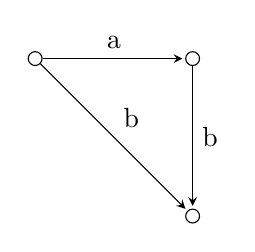
\begin{tikzpicture}[>=stealth, shorten >=1pt, auto, node distance=2cm,initial text={}]
\node[state,  inner sep=1pt, minimum size=5pt] (S0){};
\node[state,  inner sep=1pt, minimum size=5pt][right of =S0] (S1){};
\node[state,  inner sep=1pt, minimum size=5pt][below of =S1] (S2){};
\path[->](S0) edge   node {a}(S1)
	      edge  node {b}(S2)
	 (S1) edge node { b }(S2)
;
\end{tikzpicture}}

\item\alert{Finito por estados} Se $S$ e $Act$ são conjuntos finitos

 \only<2>{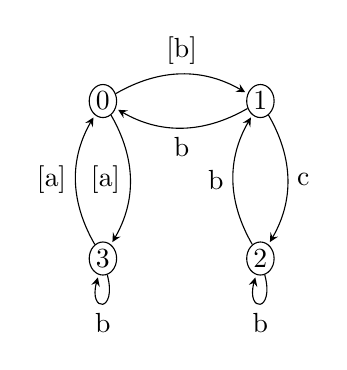
\begin{tikzpicture}[>=stealth, shorten >=1pt, auto,node distance=2cm,initial text={}]
\node[state,  inner sep=1pt, minimum size=5pt] (S0){0};
\node[state,  inner sep=1pt, minimum size=5pt][right of =S0] (S1){1};
\node[state,  inner sep=1pt, minimum size=5pt][below of =S0] (S3){3};
\node[state,  inner sep=1pt, minimum size=5pt][below of =S1] (S2){2};
\path[->](S0) edge [bend left, swap] node {[a]}(S3)
	      edge [bend left] node {[b]}(S1)
	 (S1) edge  [ bend left] node { b }(S0)
          edge  [bend left] node { c}(S2)
	(S2)  edge [loop below ] node {b}	 ()
	   edge [bend left] node {b} (S1)
	(S3)  edge [loop below ] node {b}	 ()
	   edge [bend left] node {[a]} (S0)
;
\end{tikzpicture}}

\item\alert{Ramificação-limitada} $(\exists k\geq 0)(\forall s\in S)( |Post(s)|\leq k)$

\only<3>{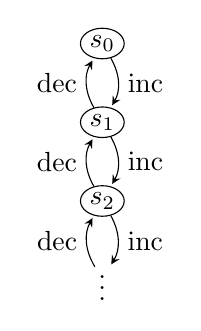
\begin{tikzpicture}[>=stealth, shorten >=1pt, auto,node distance=1cm,initial text={}]
\node[state,  inner sep=1pt, minimum size=5pt] (S0){$s_0$};
\node[state,  inner sep=1pt, minimum size=5pt][below of =S0] (S1){$s_1$};
\node[state, inner sep=1pt, minimum size=5pt][below of =S1] (S2){$s_2$};
%\node[state,  inner sep=1pt, minimum size=5pt][below of =S2] (S3){};
\node[  inner sep=1pt, minimum size=5pt][below of =S2] (S3){$\vdots$};
\path[->](S0) edge [bend left] node {inc}(S1)
	 (S1) edge  [ bend left] node { dec }(S0)
			  edge [bend left] node {inc}	 (S2)
	(S2)  edge [bend left ] node {dec}	 (S1)
 			edge [bend left] node {inc}	 (S3)
(S3)  edge [bend left ] node {dec}	 (S2);
\end{tikzpicture}

$s_n$ guarda o valor $n$ que pode ser incrementado ou decrementado de $1$. Tem grau de ramificação $2$. Não é finito por estados}

\item\alert{Finitamente Ramificado} $(\forall s\in S)(|Post(s)|\leq \infty)$. Caso contrário é infinitamente ramificado


\only<4>{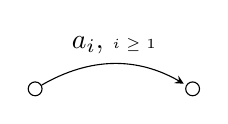
\begin{tikzpicture}[>=stealth, shorten >=1pt, auto, node distance=2cm,initial text={}]
\node[state,  inner sep=1pt, minimum size=5pt] (S0){};
\node[state,  inner sep=1pt, minimum size=5pt][right of =S0] (S1){};
\path[->](S0) edge  [bend left] node {$a_i$, \tiny{$i\geq 1$}}(S1)
;
\end{tikzpicture} 

É infinitamente ramificado}
\end{itemize}
\only<5>{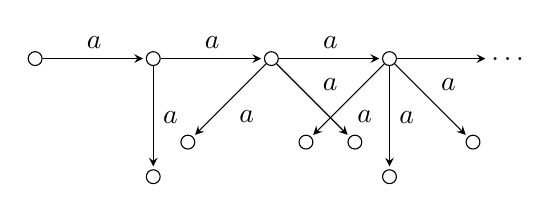
\begin{tikzpicture}[>=stealth, shorten >=1pt, auto, node distance=1.5cm,initial text={}]
\node[state,  inner sep=1pt, minimum size=5pt] (S0){};
\node[state,  inner sep=1pt, minimum size=5pt][right of =S0] (S1){};
\node[state,  inner sep=1pt, minimum size=5pt][right of =S1] (S2){};
\node[state,  inner sep=1pt, minimum size=5pt][right of =S2] (S3){};
\node[ inner sep=1pt, minimum size=5pt][right of =S3] (S4){$\ldots$};
\node[state,  inner sep=1pt, minimum size=5pt][below  of =S1] (S11){};
\node[state,  inner sep=1pt, minimum size=5pt][below right of =S2] (S21){};
\node[state,  inner sep=1pt, minimum size=5pt][below left of =S2] (S22){};
\node[state,  inner sep=1pt, minimum size=5pt][below right of =S3] (S31){};
\node[state,  inner sep=1pt, minimum size=5pt][below of =S3] (S32){};
\node[state,  inner sep=1pt, minimum size=5pt][below left of =S3] (S33){};

\path[->](S0) edge   node {$a$}(S1)
(S1) edge   node {$a$}(S2)
	edge node {$a$} (S11)
(S2) edge   node {$a$}(S3)
edge node {$a$} (S22)
edge node {$a$} (S21)
(S3) edge   node {}(S4)
edge node {$a$} (S31)
edge node {$a$} (S32)
edge node {$a$} (S33)
;
\end{tikzpicture}

Não é de ramificação limitada}

\end{frame}

\begin{frame}{Equivalência de LTSs (I)}

\begin{itemize}
	\item 
Uma questão fulcral é a de decidir quando dois LTSs são equivalentes.
\item Em princípio serão quando um observador não os consegue distinguir. \item Mas como definir isso?
Podemos obrigar a que
\begin{itemize}
\item  os LTS são isomorfos como grafos (Isomorfismo)
\item ou os LTS tenham os mesmos caminhos (Equivalência por traços (linguagens))
\item ou ...
\item iremos deixar isto para mais tarde
\end{itemize}
\end{itemize}

\end{frame}
\section{Modelação de Processos Concorrentes}

\begin{frame}{Processos Concorrentes}
\begin{itemize}[<+->]
	\item Cada processo é representado por um sistema de transições (LTS) 
\item Neste caso, o tempo avança quando se muda de estado por uma transição (execução de um programa sequencial)

\item O que acontece se executam concorrentemente?
\item Assumimos que:
\item O tempo só é considerado de forma relativa (um processo $p$  ocorre antes do processo $q$)
\item A ações são atómicas e instantâneas
\item Os processos concorrentes executam independentemente excepto se explicitamente comunicarem (coordenação)
\end{itemize}	
\end{frame}

\begin{frame}{Processos concorrentes $A$ e $X$}
\onslide<1->{
\begin{center}
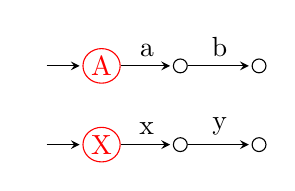
\begin{tikzpicture}[>=stealth, shorten >=1pt, auto, node distance=1cm,initial text={}]
\node[state,  inner sep=1pt, minimum size=5pt, color=red , initial] (S0){A};
\node[state,  inner sep=1pt, minimum size=5pt][right of =S0] (S1){};
\node[state,  inner sep=1pt, minimum size=5pt][right of =S1] (S2){};
\node[state,  inner sep=1pt, minimum size=5pt,  color=red , initial ] [below of =S0](T1){X};
\node[state,  inner sep=1pt, minimum size=5pt][right of =T1] (T2){};
\node[state,  inner sep=1pt, minimum size=5pt][right of =T2] (T3){};

\path[->](S0) edge node {a}(S1)
	 (S1) edge  node { b }(S2)
	(T1) edge node {x}(T2)
	 (T2) edge  node { y }(T3)
;
\end{tikzpicture}
\end{center}
}
\only<2->{

\begin{columns}
\begin{column}{0.3\textwidth}
	se $A$ executa \alert{a}
\end{column}
	
	\begin{column}{0.7\textwidth}
\begin{center}	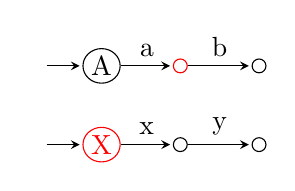
\begin{tikzpicture}[>=stealth, shorten >=1pt, auto, node distance=1cm,initial text={}]
\node[state,  inner sep=1pt, minimum size=5pt,  initial] (S0){A};
\node[state,  inner sep=1pt, minimum size=5pt , color=red][right of =S0] (S1){};
\node[state,  inner sep=1pt, minimum size=5pt][right of =S1] (S2){};
\node[state,  inner sep=1pt, minimum size=5pt,  color=red , initial ] [below of =S0](T1){X};
\node[state,  inner sep=1pt, minimum size=5pt][right of =T1] (T2){};
\node[state,  inner sep=1pt, minimum size=5pt][right of =T2] (T3){};

\path[->](S0) edge node {a}(S1)
	 (S1) edge  node { b }(S2)
	(T1) edge node {x}(T2)
	 (T2) edge  node { y }(T3)
;
\end{tikzpicture}\end{center}
\end{column}
\end{columns}
}
 

\only <3->{
\begin{columns}
\begin{column}{0.3\textwidth}
	se $X$ executa  \alert{x}
\end{column}

\begin{column}{0.7\textwidth}\begin{center}
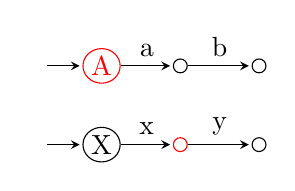
\begin{tikzpicture}[>=stealth, shorten >=1pt, auto, node distance=1cm,initial text={}]
\node[state,  inner sep=1pt, minimum size=5pt,  initial, color=red] (S0){A};
\node[state,  inner sep=1pt, minimum size=5pt ][right of =S0] (S1){};
\node[state,  inner sep=1pt, minimum size=5pt][right of =S1] (S2){};
\node[state,  inner sep=1pt, minimum size=5pt, initial ] [below of =S0](T1){X};
\node[state,  inner sep=1pt, minimum size=5pt, color=red ][right of =T1] (T2){};
\node[state,  inner sep=1pt, minimum size=5pt][right of =T2] (T3){};

\path[->](S0) edge node {a}(S1)
	 (S1) edge  node { b }(S2)
	(T1) edge node {x}(T2)
	 (T2) edge  node { y }(T3)
;
\end{tikzpicture}\end{center}
\end{column}
\end{columns}
}
\only <4->{
\begin{columns}
\begin{column}{0.3\textwidth}
 se $A$ e $X$ executam \alert{x} e  \alert{a} "simultaneamente"
\end{column}
\
\begin{column}{0.7\textwidth}
\begin{center}
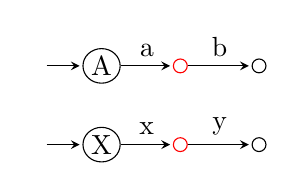
\begin{tikzpicture}[>=stealth, shorten >=1pt, auto, node distance=1cm,initial text={}]
\node[state,  inner sep=1pt, minimum size=5pt,  initial] (S0){A};
\node[state,  inner sep=1pt, minimum size=5pt , color=red][right of =S0] (S1){};
\node[state,  inner sep=1pt, minimum size=5pt][right of =S1] (S2){};
\node[state,  inner sep=1pt, minimum size=5pt, initial ] [below of =S0](T1){X};
\node[state,  inner sep=1pt, minimum size=5pt, color=red ][right of =T1] (T2){};
\node[state,  inner sep=1pt, minimum size=5pt][right of =T2] (T3){};

\path[->](S0) edge node {a}(S1)
	 (S1) edge  node { b }(S2)
	(T1) edge node {x}(T2)
	 (T2) edge  node { y }(T3)
;
\end{tikzpicture}\end{center}
\end{column}
\end{columns}
}

\end{frame}

\begin{frame}{Produto de LTS}
A execução de dois processos é um novo processo (LTS)!

\begin{center}
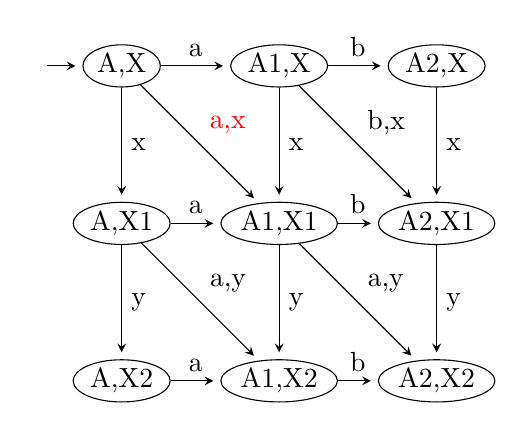
\begin{tikzpicture}[>=stealth, shorten >=2.5pt, auto, node distance=2cm,initial text={}]
\node[state,  inner sep=1pt, minimum size=5pt,  initial] (S0){A,X};
\node[state,  inner sep=1pt, minimum size=5pt][right of =S0] (S1){A1,X};
\node[state,  inner sep=1pt, minimum size=5pt][right of =S1] (S2){A2,X};
\node[state,  inner sep=1pt, minimum size=5pt ] [below of =S0](T1){A,X1};
\node[state,  inner sep=1pt, minimum size=5pt][right of =T1] (T2){A1,X1};
\node[state,  inner sep=1pt, minimum size=5pt][right of =T2] (T3){A2,X1};
\node[state,  inner sep=1pt, minimum size=5pt] [below of =T1](P1){A,X2};
\node[state,  inner sep=1pt, minimum size=5pt ][right of =P1] (P2){A1,X2};
\node[state,  inner sep=1pt, minimum size=5pt][right of =P2] (P3){A2,X2};

\path[->](S0) edge node {a}(S1)
			edge node {x} (T1)
			edge node [color=red]{ a,x} (T2)
	 (S1) edge  node { b }(S2)
			edge node {x} (T2)
			edge node {b,x} (T3)
	(S2)	edge node {x} (T3)
	(T1) edge node {a}(T2)
		 edge node {y}(P1)
		edge node {a,y} (P2)
	 (T2) edge  node { b }(T3)
		 edge node {y} (P2)
		edge node {a,y} (P3)
	(T3)  edge node {y} (P3)
(P1) edge node {a}(P2)
(P2) edge  node { b }(P3)
;
\end{tikzpicture}
	\end{center}
\end{frame}
\begin{frame}{Simultaneidade}
\begin{columns}
\begin{column}{0.5\textwidth}
	\begin{itemize}
		\item As diagonais têm conjuntos de ações (!)
\item Mas como observar que duas ações independentes ocorrem ao mesmo tempo?
\item O seu efeito corresponde a ser primeiro uma e depois outra não interessando a ordem
\item Sendo não determinístico, podemos ignorar essas transições.
\item Não são observáveis
	\end{itemize}
\end{column}
	\begin{column}{0.5\textwidth}
{\tiny
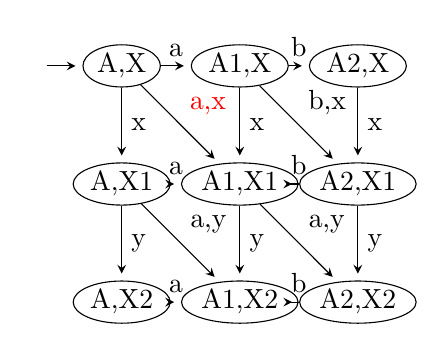
\begin{tikzpicture}[>=stealth, shorten >=2.5pt, auto, node distance=1.5cm,initial text={}]
\node[state,  inner sep=1pt, minimum size=5pt,  initial] (S0){A,X};
\node[state,  inner sep=1pt, minimum size=5pt][right of =S0] (S1){A1,X};
\node[state,  inner sep=1pt, minimum size=5pt][right of =S1] (S2){A2,X};
\node[state,  inner sep=1pt, minimum size=5pt ] [below of =S0](T1){A,X1};
\node[state,  inner sep=1pt, minimum size=5pt][right of =T1] (T2){A1,X1};
\node[state,  inner sep=1pt, minimum size=5pt][right of =T2] (T3){A2,X1};
\node[state,  inner sep=1pt, minimum size=5pt] [below of =T1](P1){A,X2};
\node[state,  inner sep=1pt, minimum size=5pt ][right of =P1] (P2){A1,X2};
\node[state,  inner sep=1pt, minimum size=5pt][right of =P2] (P3){A2,X2};
\path[->](S0) edge node {a}(S1)
			edge node {x} (T1)
			edge node [color=red]{ a,x} (T2)
	 (S1) edge  node { b }(S2)
			edge node {x} (T2)
			edge node {b,x} (T3)
	(S2)	edge node {x} (T3)
	(T1) edge node {a}(T2)
		 edge node {y}(P1)
		edge node {a,y} (P2)
	 (T2) edge  node { b }(T3)
		 edge node {y} (P2)
		edge node {a,y} (P3)
	(T3)  edge node {y} (P3)
(P1) edge node {a}(P2)
(P2) edge  node { b }(P3)
;
\end{tikzpicture}}
	\end{column}
\end{columns}
\end{frame}

\begin{frame}{Produto de LTS: sem\emph{ diagonais}}

Os estados atingíveis são os mesmos. As ações podem ocorrer por qualquer ordem (não determinismo).

\begin{center}
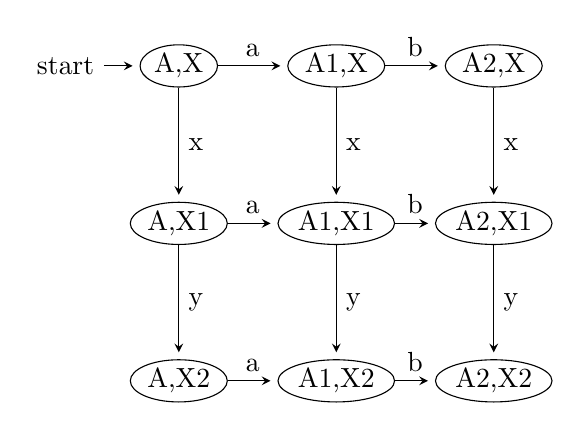
\begin{tikzpicture}[>=stealth, shorten >=2.5pt, auto, node distance=2cm]
\node[state,  inner sep=1pt, minimum size=5pt, initial] (S0){A,X};
\node[state,  inner sep=1pt, minimum size=5pt][right of =S0] (S1){A1,X};
\node[state,  inner sep=1pt, minimum size=5pt][right of =S1] (S2){A2,X};
\node[state,  inner sep=1pt, minimum size=5pt ] [below of =S0](T1){A,X1};
\node[state,  inner sep=1pt, minimum size=5pt][right of =T1] (T2){A1,X1};
\node[state,  inner sep=1pt, minimum size=5pt][right of =T2] (T3){A2,X1};
\node[state,  inner sep=1pt, minimum size=5pt] [below of =T1](P1){A,X2};
\node[state,  inner sep=1pt, minimum size=5pt ][right of =P1] (P2){A1,X2};
\node[state,  inner sep=1pt, minimum size=5pt][right of =P2] (P3){A2,X2};
\path[->](S0) edge node {a}(S1)
			edge node {x} (T1)		
	 (S1) edge  node { b }(S2)
			edge node {x} (T2)	
	(S2)	edge node {x} (T3)
	(T1) edge node {a}(T2)
		 edge node {y}(P1)
	 (T2) edge  node { b }(T3)
		 edge node {y} (P2)
	(T3)  edge node {y} (P3)
(P1) edge node {a}(P2)
(P2) edge  node { b }(P3);
\end{tikzpicture}
	\end{center}
\end{frame}

\begin{frame}{Modelo de Concorrência}
 Dados dois processos independentes a concorrência é a 
	 \alert {Intercalagem}  (\emph{interleaving/shuffle}) não-determinística de todas as ações dos dois processos.
	  
 O Diamante de intercalagem é o seguinte:
\begin{center}
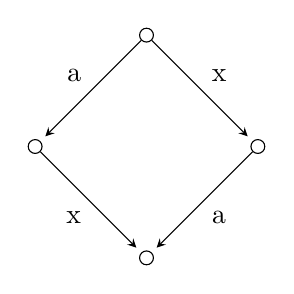
\begin{tikzpicture}[>=stealth, shorten >=2.5pt, auto, node distance=2cm,initial text={}]
\node[state,  inner sep=1pt, minimum size=5pt] (S0){};
\node[state,  inner sep=1pt, minimum size=5pt][below left of =S0] (S1){};
\node[state,  inner sep=1pt, minimum size=5pt][below right of =S0] (S2){};
\node[state,  inner sep=1pt, minimum size=5pt ] [below  right of=S1](S3){};
\path[->](S0) edge [swap] node  {a}(S1)
			edge node {x} (S2)
			
	 (S1) edge [swap] node { x }(S3)

	(S2)	edge node {a} (S3);
\end{tikzpicture}
	\end{center}

\end{frame}


\end{document}

